%
% Main document
% ===========================================================================
% This is part of the document "Project documentation template".
% Authors: brd3, ngm1, hga3, sdl3
%



%---------------------------------------------------------------------------
% define document class
%---------------------------------------------------------------------------
\documentclass[
	 a4paper			% paper format
	,10pt				% fontsize
%	,twoside			% double-sided
%	,parskip=half			% set paragraph skip to half of a line
]{scrartcl}				% KOMA-script report
%---------------------------------------------------------------------------



%---------------------------------------------------------------------------
% Set up page dimension
%---------------------------------------------------------------------------
\usepackage[
	a4paper
	,left=30mm
	,right=15mm
	,top=25mm
	,headheight=0mm
	,headsep=10mm
	,footskip=15mm
]{geometry}
%---------------------------------------------------------------------------



%---------------------------------------------------------------------------
% Load Packages:
%---------------------------------------------------------------------------
\usepackage{template/sty/bfh}
% Packages:
%---------------------------------------------------------------------------
\usepackage{fancyhdr}					% simple manipulation of header and footer
\usepackage{pdflscape}					% allow switching to landscape
\usepackage{multicol}					% allows the creation of multicols
\usepackage{chngcntr}					% allows changing the context of counters
\usepackage{pdfpages}
\usepackage[standard-baselineskips]{cmbright}		% Computer Modern Bright fonts (a family of sans serif fonts)
\usepackage[utf8]{inputenc}				% load charset UTF8
\usepackage[T1]{fontenc}				% hyphenation of words with , and
\usepackage{ae}						% better resolution of Type1-Fonts
\usepackage{graphicx}					% integration of images
\usepackage{float}					% floating objects
\usepackage{caption}					% for captions of figures and tables
\usepackage{booktabs}					% package for nicer tables
\usepackage{tocvsec2}					% provides means of controlling the sectional numbering
\usepackage{lmodern}					% use modern font
\usepackage{titlesec}
\usepackage{wrapfig}
\usepackage[export]{adjustbox}
\usepackage{lastpage}
\usepackage[ngerman, num]{isodate}
\usepackage{amsmath}					% various features to facilitate writing math formulas
\usepackage{amsthm}					% enhanced version of latex's newtheorem
\usepackage{amsfonts}					% set of miscellaneous TeX fonts that augment the standard CM
\usepackage{amssymb}					% mathematical special characters
\usepackage{exscale}					% mathematical size corresponds to textsize
\usepackage{multirow}					% multirow emables combining rows in tables
\usepackage{tabularx}
\usepackage{tcolorbox}
\usepackage{csvsimple}
\usepackage{color}
\usepackage{listings}
\usepackage[acronym, toc]{glossaries}
\usepackage{lipsum}
\usepackage{makecell}
%---------------------------------------------------------------------------
% new bibliography using biber and biblatex
%    >> breaks cite package. Patch below provides
%    >> a patch to use cite
%---------------------------------------------------------------------------
\usepackage[
    backend=biber,
    style=ieee-alphabetic,
    sortlocale=de_DE,
    natbib=true,
    url=true,
    doi=true,
    eprint=false
]{biblatex}
\usepackage{xpatch}
\makeatletter
\xpatchcmd{\@citex}{\bfseries ?}{\bfseries\expandafter\strip@prefix\meaning\@citeb}{}{}
\makeatother
%---------------------------------------------------------------------------

\usepackage{template/sty/thesis}
\usepackage{lipsum}
%---------------------------------------------------------------------------



%---------------------------------------------------------------------------
% Define document properties
%---------------------------------------------------------------------------
\newcommand{\institution}{Berner Fachhochschule}
\newcommand{\fieldofstudies}{Informatik}
\newcommand{\course}{CAS CLD FS20~ -- Cloud Computing}

\newcommand{\doctype}{Semesterarbeit}
\newcommand{\doctitle}{Informatik}
\newcommand{\docsubject}{Geodatenprozessierung mit Budget Instanzen}

\newcommand{\docauthor}{Tobias Reber}

\newcommand{\prof}{Jörg Thomann}

\newcommand{\titleImage}{hippie_car}


%---------------------------------------------------------------------------


%---------------------------------------------------------------------------
% Hyperref Package (Create links in a pdf)
%---------------------------------------------------------------------------
\usepackage[
	pdftex
	,ngerman
	,bookmarks
	,plainpages=false
	,pdfpagelabels
	,backref = {false},		% No index backreference
	,colorlinks = {true},		% Color links in a PDF
	,hypertexnames = {true},	% no failures "same page(i)"
	,bookmarksopen = {true},	% opens the bar on the left side
	,bookmarksopenlevel = {0}	% depth of opened bookmarks
	,pdftitle = {\doctitle}		% PDF-property
	,pdfauthor = {\@author}		% PDF-property
	,pdfsubject = {\docsubject}	% PDF-property
	,linkcolor = {BFHlink}		% Color of Links
	,citecolor = {BFHlink}		% Color of Cite-Links
	,urlcolor = {BFHlink}		% Color of URLs
]{hyperref}
%---------------------------------------------------------------------------


%---------------------------------------------------------------------------
% usefull commands
%---------------------------------------------------------------------------
\def\matlab{{\em MatLab}}
\def\octave{{\em Octave}}
\newcommand{\includecode}[2][c]{\lstinputlisting[caption=#2, language=#1]{#2}}
\usepackage[nottoc,notlot,notlof]{tocbibind}
\usepackage[ngerman]{babel}
%---------------------------------------------------------------------------

% ---------------------------------------------------------------------------
% Bibliography resource
% --------------------------------------------------------------------------
\addbibresource{bibliography.bib}

% ---------------------------------------------------------------------------
% Graphic paths
%---------------------------------------------------------------------------
\graphicspath{{template/}{pictures/}{svg/}}

%---------------------------------------------------------------------------
% The document
%---------------------------------------------------------------------------
\begin{document}
% Title
%---------------------------------------------------------------------------
\pagestyle{empty}
\thispagestyle{empty}

%% include BFH logo and HuCE-ml logo
\begin{figure}
	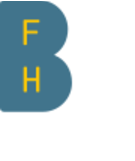
\includegraphics[scale=1,valign=t]{BFH_Logo_A_en_100_4CU.pdf}
\end{figure}

%% Document title and subtitle

\begin{minipage}[c][3cm][c]{\linewidth} {
	\centering
	\vspace*{2cm}
	{\fontsize{24pt}{0pt}\selectfont \textbf{\doctitle}}  \\
	\vspace*{0.6cm}
	{\fontsize{20pt}{0pt}\selectfont {Geodeatenprozessierung\\ mit Budget Instanzen}}  \\
	\vspace*{1cm}
	{\fontsize{14pt}{0pt}\selectfont \doctype}  \\
}
\end{minipage}


\vspace{1.5cm}


%% Title image
\begin{figure}[H]
	\centering
	\makebox[0.8\linewidth]{\color{BFHGray} \rule{0.8\linewidth}{10pt}}
	\includegraphics[width=.8\textwidth,height=9cm,keepaspectratio]{\titleImage}
	\makebox[0.8\linewidth]{\color{BFHGray} \rule{0.8\linewidth}{10pt}}
    \caption{Eine Ausfahrt mit Budget Instanzen\space\cite{HippieCar:1}}
\end{figure}

\vfill

%% Author and document information
\begin{minipage}[c][3cm][c]{\linewidth}
{
	\centering
	\begin{tabbing}
		xxxxxxxxxxxxxxxxxxx\=xxxxxxxxxxxxxxxxxxxxxxxxxxxxxxxxxxxxxxxxxxxxxxx \kill
		Departement:	\> \fieldofstudies \\
		Kurs:			\> \course \\
		Autor:		\> \docauthor \\
		Experte:		\> \prof \\
		Datum:			\> \today \\
	\end{tabbing}
}
\end{minipage}

\pagebreak


%---------------------------------------------------------------------------
% Lead
%---------------------------------------------------------------------------
\startLead
%########################################################################################################
%THE INTRO WITH Kahlil Gibran
%########################################################################################################


\newpage \vspace*{8cm}
\label{har:perplexity}
\begin{center}
\large Perplexity\\
is the beginning of knowledge.
\vspace{4mm}
\\
- Kahlil Gibran\\
\vspace{2mm}
\autocite[33]{CloudNativ:1}
\end{center}


\newpage
\section*{Management Summary}
In der Kürze liegt die Würze \autocite{DUMMY:1}

\pagebreak
\setlength{\parskip}{0pt}

%% Tabel of contents
\makeatletter
\renewcommand{\tableofcontents}{%
	\vspace*{0em}% reduce space before
	\noindent{\Large\contentsname\par}%
	\vspace{2mm}% space between title and rule
	\hrule
	\vspace{2mm}% space below rule
	\@starttoc{toc}
	\vspace{4mm}
	\hrule
}

\makeatother
\renewcommand{\contentsname}{Inhaltsverzeichnis}
\setcounter{tocdepth}{3}

\tableofcontents\label{toc}
\setlength{\parskip}{10pt}

\pagebreak

\setlength{\parskip}{0pt}

\makeatletter
\renewcommand{\listoffigures}{%
	\vspace*{0em}% reduce space before
	\noindent{\Large\listfigurename\par}%
	\vspace{2mm}% space between title and rule
	\hrule
	\vspace{2mm}% space below rule
	\@starttoc{lof}
	\vspace{4mm}
	\hrule
}

\makeatother
\renewcommand{\listfigurename}{Abbildungsverzeichnis}

\listoffigures\label{lof}
\setlength{\parskip}{10pt}

\pagebreak

%---------------------------------------------------------------------------
% Contents
%---------------------------------------------------------------------------
\startMainPart
\section{Einführung}
Der Autor arbeitet als GIS-Spezialist bei der swisstopo\footnote{\href{https://www.swisstopo.ch}{www.swisstopo.ch}}, dem Bundesamt für Landestopografie, in Wabern.\\ Unter anderem macht die swisstopo Karten. Das Team des Autoren macht Internetkarten. Lieber Leser\footnote{Im vorliegenden Dokument wurde primär eine geschlechterneutrale Formulierungen angewandt. Wo es sich nicht vermeiden liess, wurde durchwegs der männliche Singular (Leser, Benutzer) als Ansprache verwendet. Diese Ansprache bezieht sich auf beide Geschlechter sowie gegebenenfalls mehrere Personen. Sie dient lediglich der leichteren Lesbarkeit der Semesterarbeit.}, falls dir \href{https://map.geo.admin.ch}{map.geo.admin.ch} noch kein Begriff sein sollte, kann wärmstens empfohlen werden, darin zu schmökern. Die Internetkarte erfreut sich relativ grosser Beliebtheit und beinhaltet ca. 800 Themen wie Wanderwege, Solarkataster und Luftfahrthindernisse. Die Karte und die dazugehörenden Web Services sind gratis - ein Service Public der Schweizerischen Bundesverwaltung.

\begin{figure}[H]
	\centering
	\href{https://s.geo.admin.ch/8a82499889}{
	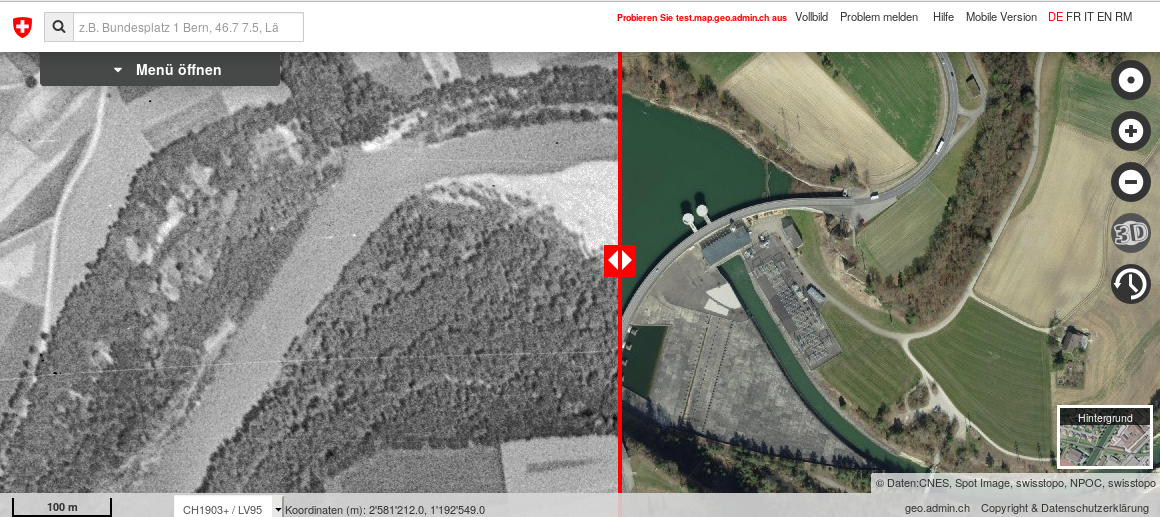
\includegraphics[width=.80\textwidth]{hist_map_geo_admin}}
	\caption{Internetkarte des Bundes \emph{\href{https://s.geo.admin.ch/8a82499889}{map.geo.admin.ch}}. Hier ein Ausschnitt der Saane bei Kleinbösingen, das Luftaufnahmen von 1946 mit heute vergleicht.}
	\label{fig:map.geo.admin.ch}
\end{figure}


\subsection{GIS - Geografische Informationssysteme}
Wie erwähnt, arbeitet der Autor als \emph{GIS-Spezialist}. Wobei ihm der Titel \emph{Geoinformatiker} besser gefällt: weil dieser Titel die Begriffe \emph{Geografie} und \emph{Informatik} vereint. \emph{Geografie} kommt aus dem Griechischen und bedeutet Erdbeschreibung \autocite[14]{Schertenleib2004}. \emph{Informatik} ist die Wissenschaft von der systematischen Darstellung, Speicherung, Verarbeitung und Übertragung von Informationen \cite{Informatik2010}.

GIS ist ein Akronym für Geografische Informationssysteme. Es bedeutet im engsten Sinn eine Ansammlung von Computerprogrammen, die zur Bearbeitung von Karten und Geodaten verwendet werden. Geodaten sind nichts weiter als Daten mit einem räumlichen Bezug\footnote{Mit Koordinaten (Nord/Ost, x/y).}. In einem weiteren Sinn deckt der Begriff GIS ein ganzes Fachgebiet ab, das sich mit Karten und Geodaten auskennt. Es ist also nicht nur ein Werkzeug, sondern ein Fachgebiet, das Kenntnisse über Datensammlung, Speicherung, Analyse und Darstellung innerhalb von vielen verschiedenen Themen mit einem räumlichen Bezug abdeckt. Typische Geodaten sind digitale Karten, Inventare und Register von Parzellen, Umweltfaktoren, Grenzen, Entwicklung, Planung etc., die einen räumlichen Bezug haben und dadurch in einem geografischen Zusammenhang analysiert und dargestellt werden können \autocite[15]{Balstroem}.

Es ist zwar weit von der klassischen Geografie zu Zeiten Alexanders von Humbold\footnote{Ein Forschungsreisender des 19 Jh. mit einem weit über Europa hinausreichenden Wirkungsfeld. Mehrjährige Forschungsreisen führten ihn nach Lateinamerika, USA und nach Zentralasien \cite{Kehlmann2005}.} entfernt, aber es liegt auf der Hand, dass auch die Geografie Cloud Computing nutzt.
\section{Vorgehen}
In diesem Kapitel wird das Vorgehen beschrieben, wie die Arbeit geplant und realisiert wurde. 

\subsection{Arbeitsmethodik}
Da die Arbeit von einem einzigen Autor umgesetzt wurde, musste bezüglich Arbeitsmethodik nur wenig definiert und koordiniert werden.

Um zu starten, hat dem Autor geholfen, dass der erste Besprechungstermin mit dem Experten bereits anfangs Sommer (16. Juli) angesetzt wurde. Um eine Diskussionsbasis für diesen Termin zu haben, musste sich der Autor ernsthaft mit der Semesterarbeit auseinandersetzen. Dazu hat er aus einer BFH Vorlage \footnote{Herzlichen Dank an Andreas Habegger und Lukas Studer fürs Bereitstellen der \href{https://gitlab.ti.bfh.ch/latex-utils/tpl_latex-thesis}{LaTex Vorlage}.} ein Gerüst der Arbeit erstellt und stichwortartig abgefüllt. Nach gründlicher Diskussion mit dem Experten wurde dieses Gerüst etwas angepasst und diente von da an als Basis für die Arbeit; wo sich die Kapitel zunehmend von losen Notizen zum finalen Zustand festigten.

Um die Übersicht der anstehenden Aufgaben nicht zu verlieren, wurde beschlossen, nach Kanban zu arbeiten. Weil für die Arbeit ein Repository auf \emph{github.com}\footnote{\href{https://github.com/bfh-semesterarbeit/spot-geoprocessing/projects/1}{Projekt auf github.com}.} angelegt wurde, konnte dort auch gleich ein Kanban Board erstellt werden. Das Kanban Board wurde vor allem dafür genutzt, fortlaufend Aufgaben zu erfassen und um die Menge der angefangenen Aufgaben zu kontrollieren. Es wurde darauf geachtet, die Menge der angefangenen Aufgaben möglichst klein zu halten.

Dadurch konnte im Alltag (wenn gerade etwas Zeit zur Verfügung stand) eine solche Aufgabe genommen und erledigt werden. Es wurde nicht strikte nach Kanban gearbeitet, aber einige Prinzipien daraus wurden verwendet. Zum Beispiel wurde das erste Grundprinzip angewendet \textit{"Beginne mit dem, was du gerade tust:
In diesem Grundprinzip stecken zwei Dinge. Indem man mit dem beginnt, was man gerade tut, beendet man die aktuelle Arbeit, bevor etwas Neues begonnen wird. Genauso ist hier aber auch die Aussage enthalten, dass Kanban einfach eingeführt werden kann."} \cite{kanban2010}. Eine Momentaufnahme des Kanbans befindet sich im Anhang \ref{appendix:kanban}.

\subsection{Projektplan}\label{chap:projektplan}
Um den übergeordneten Rahmen der Arbeit nicht aus dem Fokus zu verlieren und um sich bewusst zu machen, wieviel Zeit generell bis zur Abgabe zur Verfügung steht, war es hilfreich, einen Projektplan mit Meilensteinen zu erstellen. Durch die Berner Fachhochschule waren die grundlegenden Meilensteine bereits vorgegeben. Der Projektplan befindet sich im Anhang \ref{appendix:projektplan}.

\section{Ausgangslage}
Hier werden das Arbeitsumfeld und die Aufgaben beschrieben, aus denen sich die Problemstellung dieser Semesterarbeit ergeben hat.

\subsection{swisstopo bei AWS}
Es liegt auf der Hand, dass die swisstopo in ihrer Rolle als \emph{Geoinformationszentrum} auf Cloud Computing setzt. Die swisstopo nutzt Cloud Computing mit AWS\footnote{Amazon Web Services} seit mehr als 10 Jahren für den Betrieb des Geoportal des Bundes.
 
\textit{"Mit der BGDI\footnote{Bundesgeodateninfrastruktur: Viewer und andere Services.} unter AWS können wir derzeit ca. eine Million Internetbenutzer pro Monat bedienen. Dank AWS können wir die zur Zuordnung neuer Server benötigte Zeit erheblich verkürzen und unseren Fokus auf echte Kundenanforderungen verstärken."} \cite{Christ2020}.


\subsection{Publikation von Geodaten}
Wie bereits erwähnt, können auf dem Viewer ca. 800 Themen wie Wanderwege, Solarkataster und Luftfahrthindernisse angesehen werden. Das Team des Autoren publiziert diese Daten. Der Nachführungszyklus wie auch der Aufwand zur
Aufbereitung der Daten fürs Web sind unterschiedlich. Einige Daten werden manuell aufwändig aufbereitet, andere
stündlich automatisch nachgeführt.

\subsection{Web Services geben den Technologie Stack vor}\label{kap:webservices}
Nebst der Publikation der Daten ist das Team des Autoren für den Betrieb und der Weiterentwicklung der Web Services
und des Viewers verantwortlich. Der ganze Technologie Stack wurde schon länger nicht mehr grundlegend erneuert. Zurzeit wird
die gesamte Architektur analysiert und überarbeitet, um eine gestaffelte Migration auf eine neue
Lösung zu ermöglichen.
Einige Rahmenbedingungen dieser zukünftigen Architektur sind bereits klar: Das Geoportal des
Bundes wird weiterhin in der AWS Cloud betrieben werden, bevorzugt mit freier Software auf Linux\footnote{Freie Software \cite{FS2010} wie OpenLayers, PostGIS, Debian, Mapserver, Python Frameworks, Kubernetes etc.}, die Migration wird vor allem über Microservices gestaffelt erfolgen, diese Services werden als Docker Container laufen, Amazon Elastic Kubernetes Service wird die Orchestrierung der Container übernehmen; und für Continuous
Integration wird AWS Codebuild/Pipeline zum Einsatz kommen.

\newpage

\subsection{Exkurs 3D Daten}
Die swisstopo erfasst und aktualisiert Daten mit einem räumlichen Bezug. Diese Geodaten sind die Basis für die Ableitung in eine Vielzahl von Produkten, wie die Landeskarten 1:25'000. Nebst Karten gibt es unter anderem die Produktpalette der Landschaftsmodelle. Diese geben die Objekte der Landschaft im flexiblen Vektorformat wieder. Sie bestehen aus thematischen Ebenen (Bsp. Gebäude). Jede Ebene umfasst georeferenzierte Punkt-, Linien-, Flächen- oder 3D Objekte. Jedes Objekt enthält Attribute und Beziehungen \cite{toposhop2010}.

Zu den Landschaftsmodellen gehören Produkte wie swissTLM3D und swissBuildings3D. Im Viewer wird eine Auswahl von Themen aus eben diesen Landschaftsmodellen dargestellt: Zurzeit Gebäude, Bäume, Seilbahnen, Namen und das Terrain. Vor wenigen Jahren wurden diese 3D Daten mit einem grossen Effort medienwirksam publiziert.

\begin{figure}[H]
	\centering
	\href{https://s.geo.admin.ch/8a8ce63073}{
	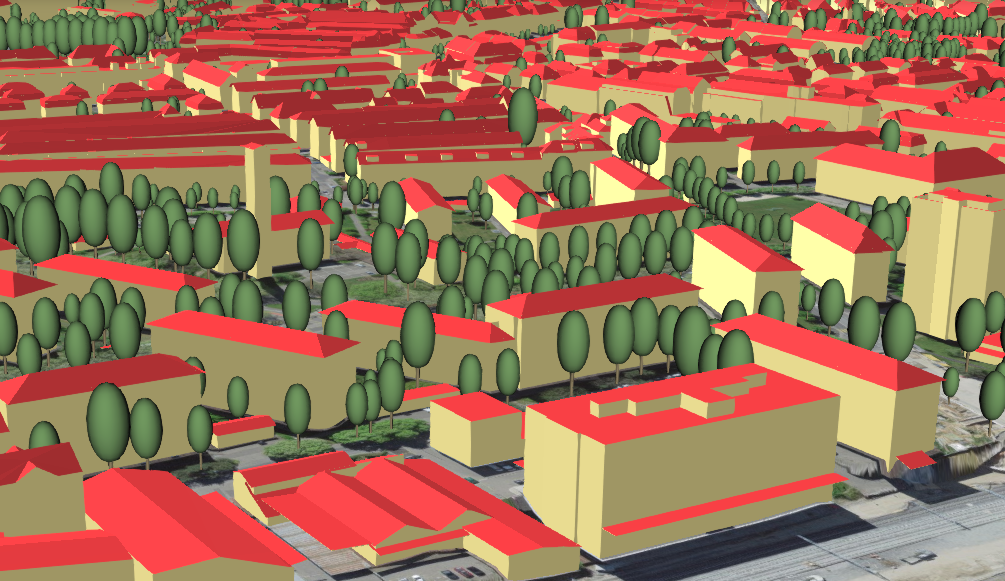
\includegraphics[width=.80\textwidth]{bfh_3d}}
	\caption{Im Viewer werden zurzeit Gebäude, Bäume, Seilbahnen, Namen und das Terrain dargestellt. Um aktuell zu bleiben, müssen diese 3D Daten regelmässig nachgeführt werden.}
	\label{fig:bfh_3d}
\end{figure}

Seit der Erstpublikation ist inzwischen etwas Zeit vergangen. Als die ersten Aktualisierungen der Daten anstanden, wurde den Beteiligten bewusst, dass sich diese nicht einfach so \emph{auf Knopfdruck} realisieren lässt: Seit der Erstpublikation hat es personelle Wechsel gegeben und bezüglich Dokumentation und Automatisierungsgrad wurden Lücken identifiziert.

Es gibt immer gute Gründe für \emph{technische Schulden}, wie in diesem Fall für positive medienwirksame Reaktionen\footnote{Wie Bsp. auf watson.ch oder Twitter \cite{watson2018}.}. Früher oder später müssen diese abgebaut werden, weil es einen direkten Einfluss auf die Wartbarkeit des Produktes hat \cite{technischeschulden2010}.

\section{Use Case}
\subsection{Problemstellung}
Es ist der swisstopo schon lange ein Anliegen, die Publikationsvorgänge von Geodaten zu optimieren. Wann immer möglich, soll der Automatisierungsgrad erhöht werden.

Besonders aufwändig erweist sich zurzeit die Publikation von 3D Daten. Die manuelle Publikation
der 3D Daten benötigt eigene Tools, die auf einem performanten und somit teuren Rechner laufen
müssen. Ausserdem erfordert die Bereitstellung einen hohen Koordinationsaufwand zwischen der
Infrastruktur und der Entwicklung. Dabei passiert es, dass Mängel in den 3D Daten erst nach
beendeter Webpublikation bemerkt werden; und der ganze Publikationsvorgang muss wieder von
vorne gestartet werden.
Auch dem Hersteller der 3D Daten (dem Bereich Topografie) wäre es ein Anliegen, wenn er diese
Daten selbst automatisch publizieren und prüfen könnte.

Einerseits soll in dieser Arbeit mittels eines Prototyps aufgezeigt werden, wie der Automatisierungsgrad erhöht werden könnte. Andererseits soll untersucht werden, ob für die Verarbeitung Budget Instanzen\footnote{Amazon Spot Instanzen} anstelle von On-Demand Instanzen\footnote{Herkömmliche EC2 Instanzen.} verwendet werden können und wie deren Einsatz aussehen könnte.

\subsubsection{Budget Instanzen}\label{kap:bugdet_instanzen}
Amazon preist Budget Instanzen folgendermassen an: \textit{"Mit Amazon EC2 Spot-Instances können Sie die Vorteile nicht genutzter EC2-Kapazitäten in der AWS Cloud nutzen. Spot-Instances sind mit einem Rabatt von bis zu\\ 90\% im Vergleich zum On-Demand-Preis verfügbar. Sie können Spot-Instances für diverse statuslose, fehlertolerante und flexible Anwendungen verwenden. Dazu zählen unter anderem Big-Data-Anwendungen, auf Containern ausgeführte Workloads, CI/CD, Webserver-Anwendungen, HPC-Anwendungen (High-Performance Computing) sowie Test- und Entwicklungs-Workloads."} \cite{AmazonAWSSpot:1}.


\begin{figure}[H]
	\centering
	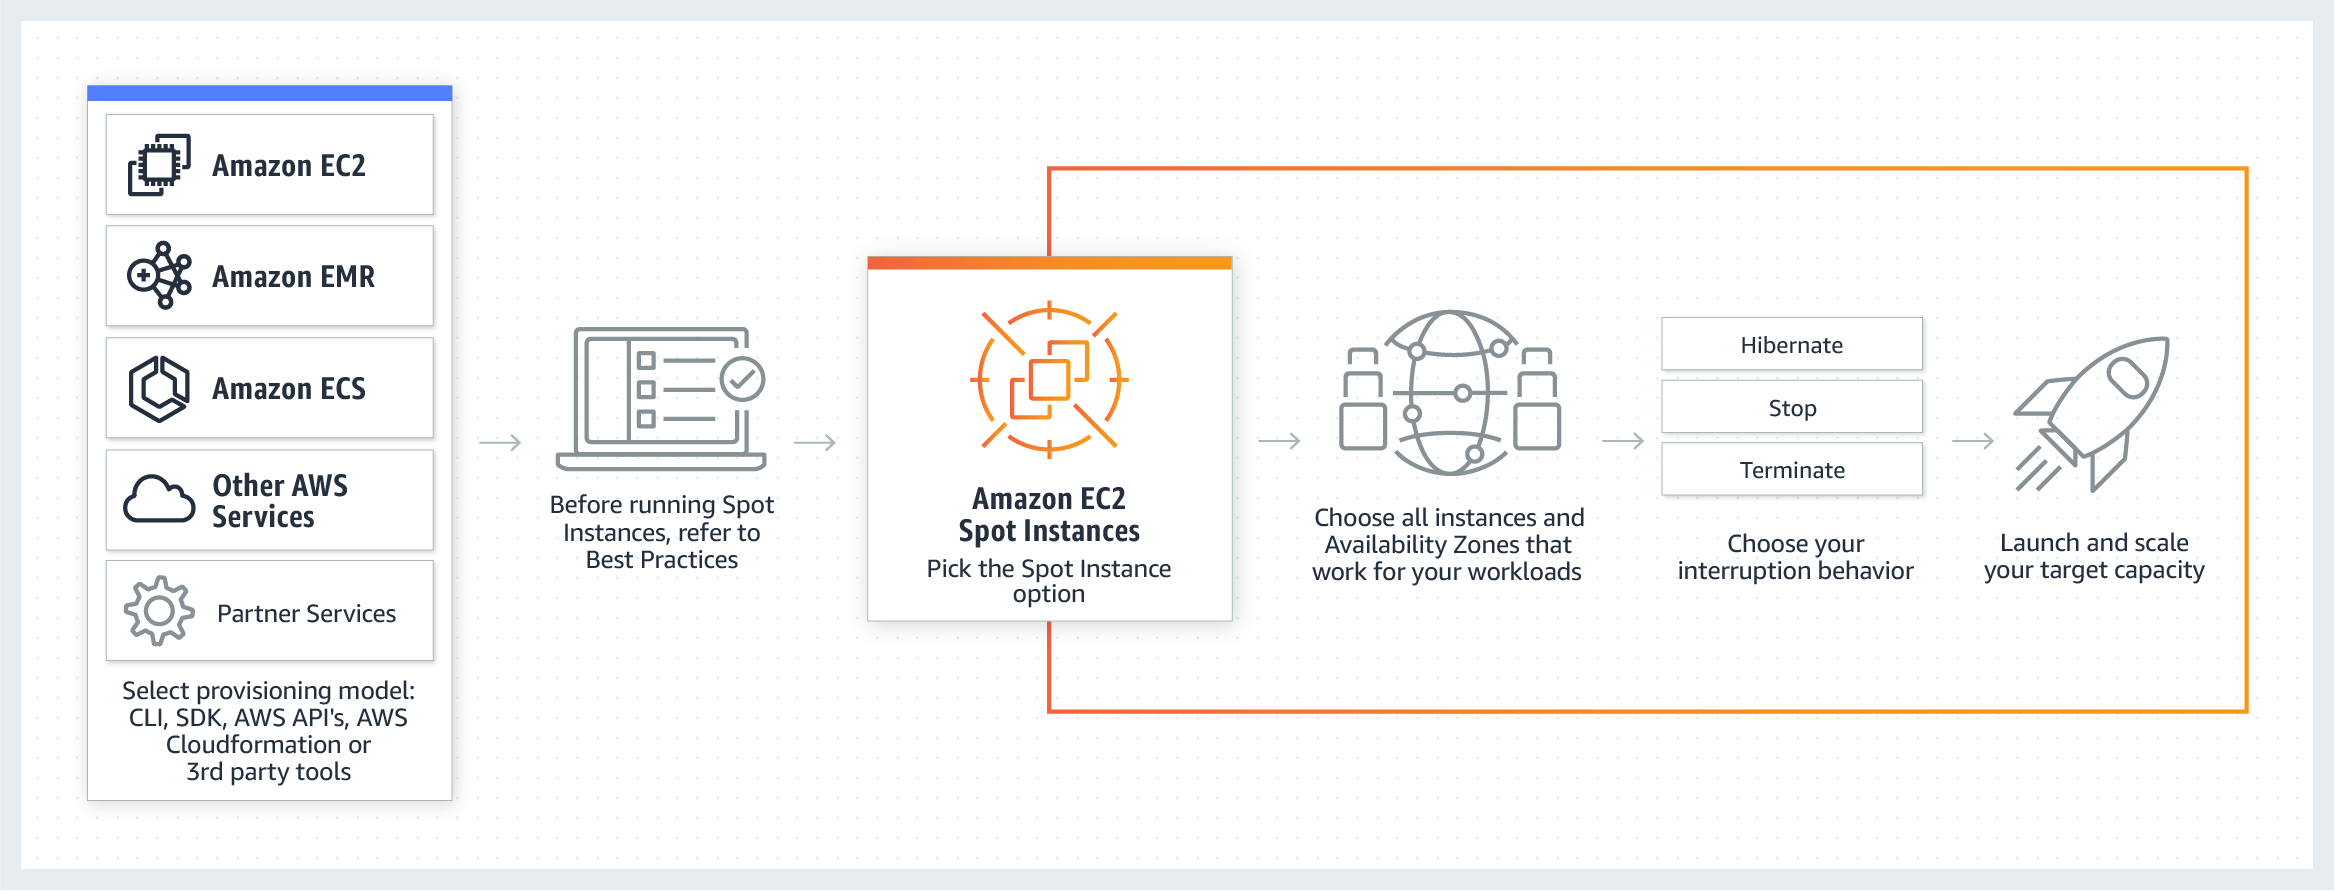
\includegraphics[width=.70\textwidth]{spot}
	\caption{So funktioniert das Ausleihen von Budget (SPOT) Instanzen}
	\label{fig:spot}
\end{figure}

Das Verkaufsargument \emph{90\%} Rabatt ist eine Ansage: Eine Preis-Aktion, ein Budget Produkt, um die Auslastung von EC2 Kapazitäten zu steigern. Der Konsument gibt viel weniger aus, mit dem Nachteil, dass ihm die Instanz innerhalb von 2-minütiger Vorankündigung weggenommen werden kann \cite{AmazonAWSSpot:1}.

Möchte man die EC2 Spot Instanzen für die Geodatenverarbeitung einsetzen, muss also ein Weg gefunden werden, um mit diesen Unterbrüchen umgehen zu können.

Wie auf der Abbildung \ref{fig:spot} dargestellt, kann das Verhalten der Instanz bei einem Interrupt\footnote{Wenn Amazon die Spot Instanz für einen anderen Zweck beanspruchen möchte, die wegnimmt.} definiert werden. Es besteht dabei sogar die Möglichkeit eines \emph{Hibernate}, das den Zustand des RAMs vor dem Unterbruch auf der Festplatte abspeichert.

Diese 2-minütige Vorankündigung eines Interrupts kann auch via RESTful Abfrage\footnote{EC2 Spot Instance Interruption Notice, eine HTTP Abfrage: Im Anhang \ref{appendix:restful} hat es ein Beispiel dazu.} von der Instanz aus abgefragt werden.

Diese Vorankündigung lässt sich auch via AWS CLI abfragen. In einem grösseren Setup könnte das Signal der Vorankündigung auch mit dem AWS Überwachungstool \emph{CloudWatch} verarbeitet werden.


\subsection{Ist-Zustand der 3D Datenpublikation}
\subsubsection{3D Datenpublikation}
Das Aufzeigen des Ist-Zustandes soll helfen, einen generellen Überblick der Aufgaben und Teile zu schaffen, die es braucht, um 3D Daten zu Publizieren. Es bildet die Grundlage, um die Frage zu beantworten, welche Arbeiten erledigt werden müssen, um die 3D Daten im Web zu publizieren? Welche Arbeitsschritte könnten automatisiert werden? 

Eine Datenpublikation läuft folgendermassen ab: Sobald der Auftrag für eine 3D Datenpublikation erteilt wurde\footnote{Vom Bereich Topografie.}, müssen zurzeit folgende Schritte, die in der Abbildung \ref{fig:ist_zustand} referenziert sind, erledigt werden:

\begin{figure}[H]
	\centering
	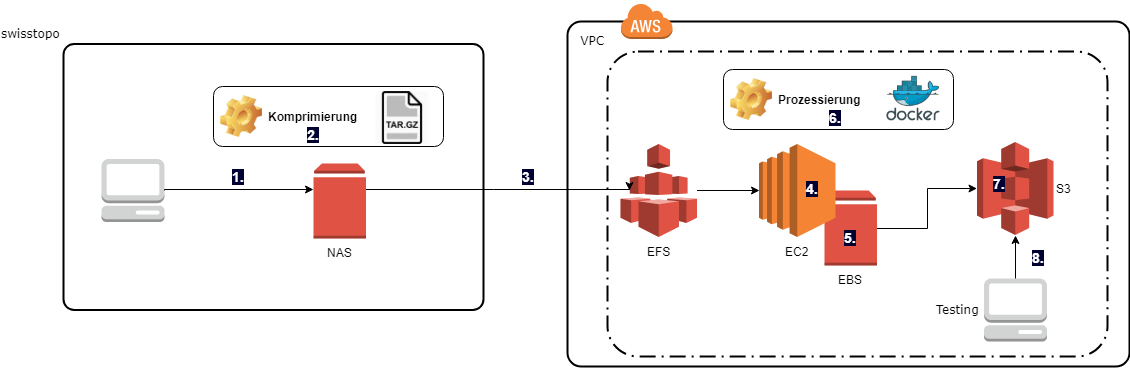
\includegraphics[width=1.0\textwidth]{ist_zustand}
	\caption{Arbeitsschritte, die es braucht, um die 3D Daten zu Publizieren.}
	\label{fig:ist_zustand}
\end{figure}

\begin{enumerate}
\item Die Rohdaten\footnote{Das Format der Rohdaten ist KML/COLLADA (beides XML).} werden vom Auftraggeber (Bereich Topografie) auf einem NAS bereitgestellt.
\item Da es sich um ca. 8 Millionen Dateien handelt, werden diese je Kartenblatt\footnote{Blatteinteilung: Die swisstopo arbeitet viel nach Blatteinteilung nach Kartenblättern, hier ein Beispiel: \href{https://s.geo.admin.ch/8b5f3f6721}{map.geo.admin.ch}.} erst einmal komprimiert, um so (weil bedeutend weniger Dateien) schneller kopiert werden zu können.
\item Kopieren\footnote{Via \emph{rsync}.} der komprimierten Dateien vom swisstopo Netzwerk in die Amazon Cloud (AWS VPC\footnote{AWS: Amazon Web Services, VPC: Virtual Private Network.}).
\item Parallel dazu wird die IT via Ticket gebeten, eine Instanz mit entsprechendem Image\footnote{Eine EC2 Instanz aus einem bereits vorhandenen AMIs.} bereitzustellen.
\item Kopieren und Entpacken der Rohdaten auf die gemountete Festplatte\footnote{Ein EBS Volumen.} des Servers.
\item Die Daten auf dem Server via Docker verarbeiten\footnote{Umwandeln in das Web Format \emph{Cesium3DTiles}.}.
\item Kopieren der Web-optimierten Daten auf S3.
\item Die Daten visualisieren, um sie inhaltlich prüfen zu können. Ein Codepen Projekt\footnote{SaaS: Eine Webseite, um Front-End Code zu schreiben, zu testen, und bereitzustellen (\href{https://codepen.io}{codepen.io}).}, dass auf die 3D Tiles zugreift.
\end{enumerate}

\subsubsection{Aufwand der Verarbeitung}
\label{aufwand_prozessierung}
Folgende Schritte sind besonders aufwendig:
\begin{itemize}
\item \textbf{Abb. \ref{fig:ist_zustand}, Schritt 2. und 5.}: Das Kopieren / Komprimieren (Packen und Entpacken) der Rohdaten dauert lange.
\item Es kann vorkommen, dass Daten korrupt sind. Dies führt zu Teillieferungen, mit der Gefahr, dass zu einem Durcheinander der einzelnen Teillieferungen kommen könnte.
\item \textbf{Abb. \ref{fig:ist_zustand}, Schritt 4.}: Die IT muss für die Verarbeitung eine EC2 Instanz mit entsprechendem Volumen bereitzustellen. Um laufende Kosten zu verringern, wird diese Instanz nach getaner Arbeit\footnote{Der Verarbeitung.} wieder gestoppt. Falls mit den Daten etwas nicht in Ordnung ist, muss dieser Schritt von der IT wiederholt werden. Ausserdem muss auf der Instanz noch das eine oder andere manuell installiert und konfiguriert werden.
\end{itemize}

\subsubsection{Technische Komponenten}
Auflistung der technischen Komponenten:
\begin{itemize}
\item \textbf{Abb. \ref{fig:ist_zustand}, Schritt 2., 3. und 5.}: Das Komprimieren und Kopieren der Rohdaten erfolgt mit Linux Bordmitteln (\emph{cp}, \emph{rsync}, \emph{tar}).
\item \textbf{Abb. \ref{fig:ist_zustand}, Schritt 4. und 7.}: Erfolgen via AWS CLI.
\item \textbf{Abb. \ref{fig:ist_zustand}, Schritt 6.}: Via Docker. Der Container wurde von der Firma Analytical Graphics Inc. \cite{AGI2010} bereitgestellt. Das Tool, das die Rohdaten in ein Web-Format umwandelt, wird mit Node.js ausgeführt.
\item \textbf{Abb. \ref{fig:ist_zustand}, Schritt 7.}: Ein Projekt, um die Daten im Browser betrachten und inhaltlich Testen zu können, erfolgt über die Webseite codepen.io.
\end{itemize}



\section{Architektur}
Ausfindigmachen von verschiedenen Architekturen
\subsection{Bewertungskriterien}
\begin{itemize}
\item Muss in AWS Cloud
\item Zugang zu EFS
\item Automatisierbar sein
\end{itemize}
\subsection{Variante 1: Spot}
Evtl. lässt sich eine Lösung finden ohne EKS zu verwenden

\subsection{Variante 2: Spot mit EKS}
Spot mit EKS
\section{Prototyp}
\subsection{Realisierung}
Für die Realisierung des Prototypen hat der Autor das Kennenlern-Angebot von AWS, ein einjähriges kostenloses Kontingent an Services und Produkten\cite{FreeTier2020}, gewählt. 

Nachdem der \emph{AWS Testaccount} erstellt war, mussten erste Schritte wie grundlegende Konfigurationen des Identity Access Management (IAM) gemacht und das Steuern von Spot Anfragen erlernt werden.

Weitere Schritte folgten. Die Realisierung des Prototypen wird in den folgenden Kapiteln beschrieben werden.

\begin{figure}[H]
	\centering
	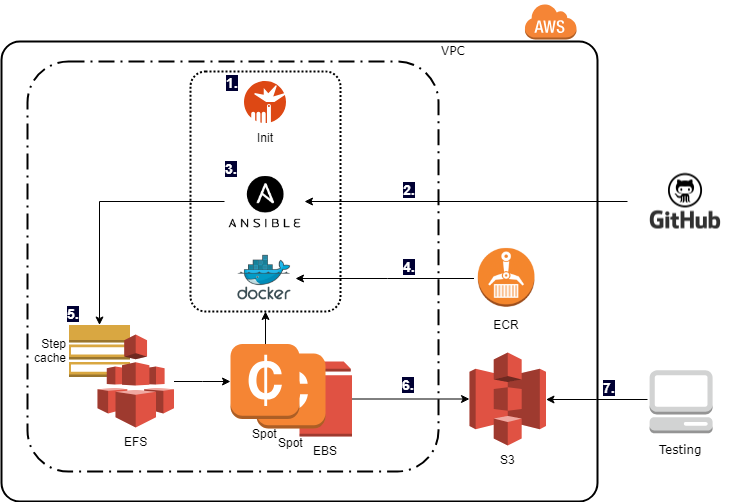
\includegraphics[width=.90\textwidth]{poc_zustand}
	\caption{Geodatenprozessierung mit SPOT Instanzen.}
	\label{fig:ist_zustand}
\end{figure}

\subsubsection{Der Publikationsvorgang als Code}
Mit der Entscheidung, die Spot Instanz via \emph{Cloud-Init}-Ansatz (Abb. \ref{fig:ist_zustand}, Nr. 1) mit Ansible zu Provisionieren\footnote{Und nicht via einem neuen AMI.}, lag es auf der Hand auch gleich Ansible für den Publikationsvorgang zu verwenden (Nr. 3).

Das Init-Skript wie auch die Ansible Deklarationen können \href{https://github.com/bfh-semesterarbeit/up-and-running-dataprocessing}{auf github.com/bfh-semesterarbeit} angeschaut werden.




\subsubsection{Handling der Interrupts}
Sämtliche Schritte werden via Ansible verwaltet und sobald ein Schritt erledigt wurde, hält Ansible dies auf dem gemounteten EFS Volumen in einer Textdatei fest.

Falls es zu einem Interrupt kommen sollte, wird von der Spot Flotte die nächste Instanz bereitgestellt und Ansible macht bei dem Schritt weiter, der zuletzt in der Textdatei festgehalten wurde (Abbildung \ref{fig:ist_zustand}, Nr. 5).


\subsection{Testen}

\paragraph{Testen der Datenstruktur}


\paragraph{Unerwartetes Herunterfahren}


\paragraph{Real Case Szenario}

Der komplette Rohdatensatz, alle Gebäude der Schweiz, wurde prozessiert. Das Resultat kann vorläufig\footnote{Bis am 1. November 2020} hier betrachtet werden:
\href{https://codepen.io/rebert/pen/ExKZmmE}{https://codepen.io/rebert/pen/ExKZmmE} Wobei nur die Gebäude vom S3 Testbucket kommen (Abb. \ref{fig:ist_zustand}, Nr. 7) 

\section{Evaluation}
\subsection{Erfahrungen}
Die Anregungen aus dem Studium\footnote{CAS in Cloud Computing an der BFH Bern: Beispielsweise die Vorlesungen Architektur, IaaS, PaaS, Docker und Kubernetes.} und das günstige Angebot von AWS haben den Autor motiviert, die komplette Infrastruktur für den Prototypen in einem eigenen AWS Account aufzubauen. Da die Infrastruktur und die Verarbeitung deklarativ festgehalten wurden, kann der Code ohne grosse Anpassungen im Account des Betriebes wiederverwendet werden.

Der Autor hat sich bewusst dazu entschieden, die Arbeit möglichst selbständig zu realisieren und hat die Ressourcen im Team und in der IT-Abteilung der swisstopo so wenig wie möglich genutzt. Es war für den Autor schon nur eine Hilfe, zu wissen, dass die Möglichkeit einer Unterstützung da war. Dies führte dazu, dass der Autor Momente der Ratlosigkeit erleben musste\ref{har:perplexity}. Was nicht weiter schlimm war, da \textit{"Perplexity is the beginning of knowledge"} \autocite[33]{CloudNativ:1}.

In der Webkonsole kann die Aufgabenart der Spot Instanz gewählt werden. Es wurden \emph{Flexible Workloads} gewählt, was möglicherweise eine gute Wahl war. Denn der Autor war darüber erstaunt, dass ihm während der gesamten Entwicklungs- und Testphase nicht ein einziges Mal eine Instanz weggenommen wurde. Die Spot Flotte musste aufgrund eines gemounteten EBS Volumens auf eine bestimmte Availability Zone beschränkt werden. Nicht einmal mit dieser Einschränkung ist es zu einem Interrupt gekommen. Um das Verhalten bei Interrupts testen zu können, mussten die Spot Instanzen somit mutmasslich terminiert werden.


\subsection{Wirtschaftlichkeit}\label{kap:wirtschaftlichkeit}
\paragraph{Personalstunden}
Der Grad der Automatisierung konnte erheblich erhöht werden. Dadurch fallen Personalstunden\footnote{In unserem Team.} weg. Vor allem diese Kosten rechnen sich. Die Verarbeitungsschritte sind im Code abgebildet, was die Fehleranfälligkeit kleiner macht, als wenn Kommandos aus der Prozessdokumentation kopiert und angepasst werden müssen. Um die IT-Abteilung gänzlich zu entlasten, müsste noch eine Rolle eingerichtet werden, die eine vordefinierte Spot Flottenanfrage steuern kann.
\paragraph{Einsparungen Spot im Vergleich zu On-Demand}
Um die Kosten von On-Demand mit Spot Instanzen zu vergleichen, werden hier die Ergebnisse des Prototyps aufgelistet. Die Verarbeitung der Gebäude mit der Mindestanforderung: 16 CPUs und 60 GB Memory. Die Gesamtrechenzeit war ca. 18 Stunden und es konnten 76\% der Kosten eingespart werden.

\begin{table}[!htbp]
\begin{center}
\begin{tabular}{| c | c | c |}
    \hline
	\textbf{Rechenzeit} & \textbf{On-Demand} & \textbf{Spot}\\
	\hline
	 \textbf{Pro Stunde} & 1.19\$ & 0.29\$\\
	\hline
	 \textbf{Total: 18 h} & 21.42\$ & 5.22\$\\
	\hline
\end{tabular}
\caption{\label{tab:price_difference}Relativ betrachtet ist das Sparpotential enorm: 76\%.}
\end{center}
\end{table}

Schaut man die Kosten relativ an, ist das Sparpotential enorm: 76\%! In absoluten Zahlen erscheint das Sparpotential für einen einzelnen Verarbeitungsauftrag nicht riesig: ca. 15\$. Dazu muss allerdings ergänzt werden, dass die Verarbeitungszeit durch die Automatisierung verkürzt wurde. Ausserdem werden jährlich mehrere 3D Updates in Auftrag gegeben. Der aufwändigste Auftrag davon ist das Update des 3D Terrains, das eine wesentlich grössere Instanz über eine längere Zeitspanne\footnote{Ca. 1 Woche.} in Anspruch nimmt.

Während der Entwicklung hat der Autor offenbar das kostenlose Kontingent einiger Dienste überschritten\footnote{Eigentlich hätte sich der Autor etwas genauer mit den Limiten der kostenlosen Kontingenten auseinandersetzen sollen. Es sind nur kleine EC2 Instanzen \emph{t2.micro} gratis (Free trier eligible).} und so wurden Anteile davon in Rechnung gestellt. Für die ganze Entwicklungsphase wurden 67\$ für Spot Instanzen verrechnet. Geht man davon aus, dass die durchschnittliche Vergünstigung gegenüber On-Demand Instanzen bei 76\% liegt, dann konnten durch das Verwenden von Spot Instanzen ca. 200\$\footnote{24\% = 67\$, 100\% = 279\$ \blacktriangleright 279\$ - 67\$ = \underline{212\$ }.} eingespart werden. 

\subsection{Kritische Punkte}

\subsubsection{Security}
Bezüglich IAM hat der Prototyp noch technische Schulden. Dem Autor ist bewusst, dass folgende zwei Sicherheitslücken bezüglich den Zugängen vorhanden sind:
\paragraph{GitHub:} Der Einfachheit halber wurde das GitHub Repository, auf welchem sich das Init-Skript und das Ansible Playbook befinden, öffentlich zugänglich gemacht (Abb. \ref{fig:ist_zustand}, Nr. 2). Dies ist nicht weiter problematisch, da der Code auf GitHub keine Passwörter etc. bekannt gibt. Aber es sind darin Informationen über die AWS Infrastruktur enthalten. Sauber wäre eine Implementation, die mit GitHub Zugangsdaten eines privaten Repositories umgehen kann. Geeignet dazu wäre z.B. der AWS Secrets Manager \cite{Secrets2020}.
\paragraph{AWS Key:} Eigens für das Kopieren auf S3, dem Zugang für die Container Registry (ECR) und für das Mounten eines SSD Volumen wurde eine IAM Rolle angelegt, die nicht mehr darf als die eben erwähnten Tätigkeiten (Abb. \ref{fig:ist_zustand}, Nr. 4 u. Nr. 6). Der Zugangsschlüssel dazu wurden auf dem EFS Volumen abgelegt. Zwar ist die Sicherheitsgruppe des EFS so konfiguriert, dass nur die Sicherheitsgruppe der EC2 Instanzen darauf Zugriff haben sollten. Trotzdem ist es nicht ideal, wenn unverschlüsselte Keys auf dem Filesystem abgelegt werden.

Sollte der Prototyp in den Betrieb überführt werden, müsste man das IAM der swisstopo übernehmen; und dieses Kapitel hätte sich erübrigt.

\subsubsection{Datenverarbeitung als Blackbox}
Idealerweise wird die Datenverarbeitung in kleine parallelisierbare und in sich selbst geschlossene Schritte unterteilt. Nach einem Interrupt der Instanz können dann die noch nicht abgeschlossenen Schritte fortgeführt werden. 

Beim gewählten Use Case der 3D Datenverarbeitung handelt es sich um eine Blackbox in einem Container, die entweder Alles oder Nichts verarbeitet. Was in diesem Fall alle (erfassten) Gebäude der Schweiz bedeutet. Damit der Prototyp funktioniert, müssen die Spot Instanzen mindestens 10 Stunden ohne Interrupt laufen. Zum Glück verhalten sich die Spot Instanzen in der Regel stabil genug, um die einzelnen langwierigen Schritte seriell verarbeiten zu können.

Der Test, der die Rohdaten auf well-formed XML testet, hilft Fehler, vor dem langwierigen Verarbeiten in der Blackbox, abzufangen. Jedoch leider nicht alle Fehler. Wenn man nun davon ausgeht, dass es in den ca. 8 Millionen Gebäuden, die geliefert wurden, immer mal wieder fehlerhafte Daten hat, welche die Blackbox ins Straucheln bringen, kann die 3D Datenverarbeitung trotz aller Automaistation zu einem mühseligen Unterfangen werden.

\section{Ausblick}
Bald steht das nächste 3D Update vor der Tür. Bei dieser Gelegenheit könnte der Automatisierungsteil dieser Semesterarbeit übernommen werden. Da es sich dabei um ein Ansible Playbook in einer deklarativen Sprache handelt, sind die einzelnen Verarbeitungsschritte auch gleich dokumentiert. Anpassungen sind einfach zu machen. Falls diese Nachführung auf einer herkömmlichen On-Demand EC2 Instanz gemacht werden müsste, könnte das Skript dennoch verwendet werden.

Mittelfristig wäre es schon nur aus Gründen des Kostensparens interessant, wenn rechenintensive Geodatenverarbeitungen auf Spot Instanzen laufen könnten. Hier nochmals: Relative Einsparungen von mehr als 70\% sind möglich; was sich mit der Zeit auch in absoluten Kosteneinsparungen (\$) sehen lassen würde.\\ Um den Koordinationsaufwand mit der IT zu verringern, könnte die Person, die eine Spot Instanz braucht, mit den nötigen Rechten versehen werden: Beispielsweise könnte sie, wie bei einem Load-Balancer, die Anzahl Instanzen der Spot Flotte von 0 auf 1 ändern dürfen, um nach getaner Arbeit die Anzahl Instanzen wieder auf 0 zu setzen.

Sobald die swisstopo über eine Hybrid Cloud verfügt, könnte die Topografie neue Daten direkt auf das EFS schreiben. Dieser Event könnte getriggert werden, um eine Spot Instanz für die 3D Geodatenverarbeitung zu starten. Jeweils ca. 18 Stunden später wären die Daten im Web und die Topografie könnte diese auf der Testumgebung einsehen (Abb. \ref{fig:ist_zustand}, Nr. 7). Diesen Vorgang könnte die Topografie solange wiederholen, bis sie mit dem Resultat zufrieden ist.

Persönlich hat dem Autor die Tour mit Spot Instanzen Spass gemacht. Die auf der Tour gemachten Erfahrungen waren ein guter Einstieg, um Services der AWS Cloud besser verstehen und nutzen zu können. Es wird sicher nicht bei dieser Tour bleiben.

\vspace{4cm}
\textit{Dank an \prof, für die Begleitung durch diese Semesterarbeit.}


%\section{Samples}
This is an example document 
\lipsum[1-3]

\clearpage
\section{Images}
\begin{figure}[H]
	\centering
	
\includegraphics[width=.6\textwidth]{placeholder}
	\caption{Overview of the frames used}
	\label{fig:placeholder}
\end{figure}

\begin{multicols}{2}
	\begin{figure}[H]
		\centering
		
\includegraphics[width=.45\textwidth,angle=90]{placeholder}
		\caption{PCB design in 3D (top view)}
		\label{fig:multicol:placeholder1}
	\end{figure}

	\begin{figure}[H]
		\centering
		
\includegraphics[width=.45\textwidth]{placeholder}
		\caption{PCB design in 3D (bottom view)}
		\label{fig:multicol:placeholder2}
	\end{figure}
\end{multicols}


\section{Table}
\begin{center}
	\begin{tabular}{ | l | l | l | p{5cm} |}
		\hline
		Day & Min Temp & Max Temp & Summary \\ \hline
		Monday & 11C & 22C & A clear day with lots of sunshine.  
		However, the strong breeze will bring down the temperatures. \\ \hline
		Tuesday & 9C & 19C & Cloudy with rain, across many northern regions. Clear spells 
		across most of Scotland and Northern Ireland, 
		but rain reaching the far northwest. \\ \hline
		Wednesday & 10C & 21C & Rain will still linger for the morning. 
		Conditions will improve by early afternoon and continue 
		throughout the evening. \\
		\hline
	\end{tabular}
\end{center}

%\begin{center}
%	\begin{tabular}{l|c}%
%		\bfseries Person & \bfseries Matr.~No.% specify table head
%		\csvreader[head to column names]{grade.csv}{}% use head of csv as column names
%		{\\\hline\givenname\ \name & \matriculation}% specify your coloumns here
%	\end{tabular}
%\end{center}

\subsection{Testing}
Dies ist der Unterttitel

\section{Lists}
\begin{itemize}
	\item sample list item
\end{itemize}

\begin{enumerate}
	\item sample list item
\end{enumerate}

\section{Code}
\begin{lstlisting}
touch --help
nano --help
mkdir --help
\end{lstlisting}

\lstinputlisting[language=C,caption=Sample C Code]{src/sampleCode.c}


\section{Equations}
This is an equation: $F = m \cdot a$

Here are some more:
\begin{align}
	y &= mx + b \\
	c^2 &= a^2 + b^2
\end{align}

and even more:
\begin{align*}
	y &= mx + b \\
	c^2 &= a^2 + b^2
\end{align*}




%---------------------------------------------------------------------------
% Bibliography
%---------------------------------------------------------------------------
\cleardoublepage
\phantomsection
\addcontentsline{toc}{section}{Literaturverzeichnis}
\renewcommand{\refname}{Literaturverzeichnis}
\printbibliography


%---------------------------------------------------------------------------
% Appendix
%---------------------------------------------------------------------------
\appendix
\startAppendix
\section{Fachbegriffe und Abkürzungen}
\begin{table}[!htbp]
\begin{tabular}{p{0.2\textwidth}p{0.7\textwidth}}
    \textbf{Abkürzung} & \textbf{Definition}\\
    \textbf{Ansible} & \makecell[l]{Ein Open-Source Automatisierungs-Werkzeug zur Orchestrierung\\ und allgemeinen Konfiguration und Administration von Computern.}\\
    \textbf{AMI} & Amazon Machine Images: Images für virtuelle Server.\\
    \textbf{Availability Zone} & \makecell[l]{Jeder Amazon Rechenzentrumstandort (Region)\\
    besteht aus mehreren isolierten Zonen, den Availability Zones.}\\
    \textbf{AWS} & Amazon Web Services\\
    \textbf{AWS CLI} & Das Command Line Interface, um AWS Ressourcen zu verwalten.\\
    \textbf{BGDI} & Bundesgeodateninfrastruktur.\\
    \textbf{Budget Instanzen} & Im Kontext dieser Arbeit ein Synonym für AWS Spot Instanzen.\\
    \textbf{EBS} & Block Storage: Speicher (für eine Instanz).\\
    \textbf{EC2} & Amazon Elastic Compute Cloud: Rechenkapazität, Speicher (und mehr).\\
    \textbf{EFS} & Amazon Elastic File System: Cloud NFS-Dateisystem.\\
    \textbf{Hybrid Cloud} & Eine Computerinfrastruktur, die Public Cloud und Private Cloud kombiniert nutzt.\\
    \textbf{IaaS} & Cloud Infrastructure as a Service: Infrastruktur \emph{"Pay as you go"} beziehen.\\
    \textbf{IAM} & Identity and Access Management: Verwaltung der Zugänge und der dazugehörenden Rechte.\\
    \makecell[l]{\textbf{On-Demand}\\ \textbf{Instanzen}} & \makecell[l]{Herkömmliche EC2 Instanzen. Der Begriff wird in dieser Arbeit manchmal\\ verwendet, um von EC2 Spot Instanzen unterscheiden zu können.}\\
    \textbf{Kartenblatt} & \makecell[l]{In der swisstopo wird viel in der Einheit von Kartenblättern gearbeitet,\\ welche die ganze Schweiz abdecken. Hier ein Beispiel: \href{https://s.geo.admin.ch/8b5f3f6721}{map.geo.admin.ch}.}\\
	\textbf{PaaS} & Plattform as a Service\\
	\textbf{POC} & Proof of Concept: Die Machbarkeit eines Produktes oder einer Idee aufzeigen.\\
	\makecell[l]{\textbf{S3}} & \makecell[l]{Amazon S3 (Simple Storage Service): Ein Filehosting-Dienst dessen Zugriff\\ über HTTP/HTTPS erfolgt.}\\
	\textbf{SaaS} & Software as a Service\\
	\textbf{SSD} &  Solid-State-Disk - Halbleiterlaufwerk: Festplatte ohne bewegliche Teile, dafür mit kurzen Zugriffszeiten.\\
	\textbf{SSH} & \makecell[l]{Secure Shell: Netzwerkprotokoll, um auf auf einen entfernten Rechner\\ zuzugreifen.}\\
	\textbf{S3} & Simple Storage Service: Ein Objektspeicherservice von Amazon.\\
\end{tabular}
\caption{\label{tab:fachbegriffe}In der Arbeit verwendete Fachbegriffe und Abkürzungen}
\end{table}
\section{Konfigurationen}
\appendCode{c}{Sample Code}{src/sampleCode.c}
\section{Kanban}\label{appendix:kanban}
\begin{figure}[H]
	\centering
	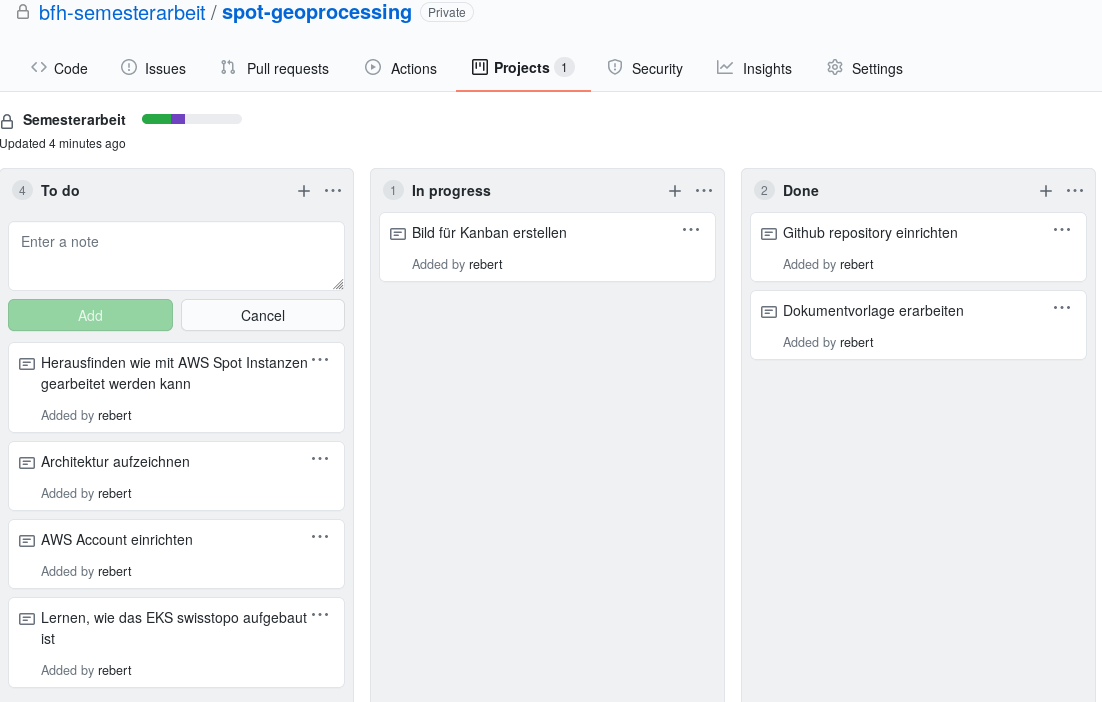
\includegraphics[width=.95\textwidth]{kanban}
	\caption{Klassisches Kanban auf \emph{github.com}}
	\label{fig:Klassisches Kanban}
\end{figure}

\section{Projektplan}\label{appendix:projektplan}
\begin{figure}[H]
	\centering
	\href{https://docs.google.com/spreadsheets/d/1zKTZgt4BW736G0xRfU9o3vWYwAJj-8nzFvGsPR7yJ_0/edit?usp=sharing}{
	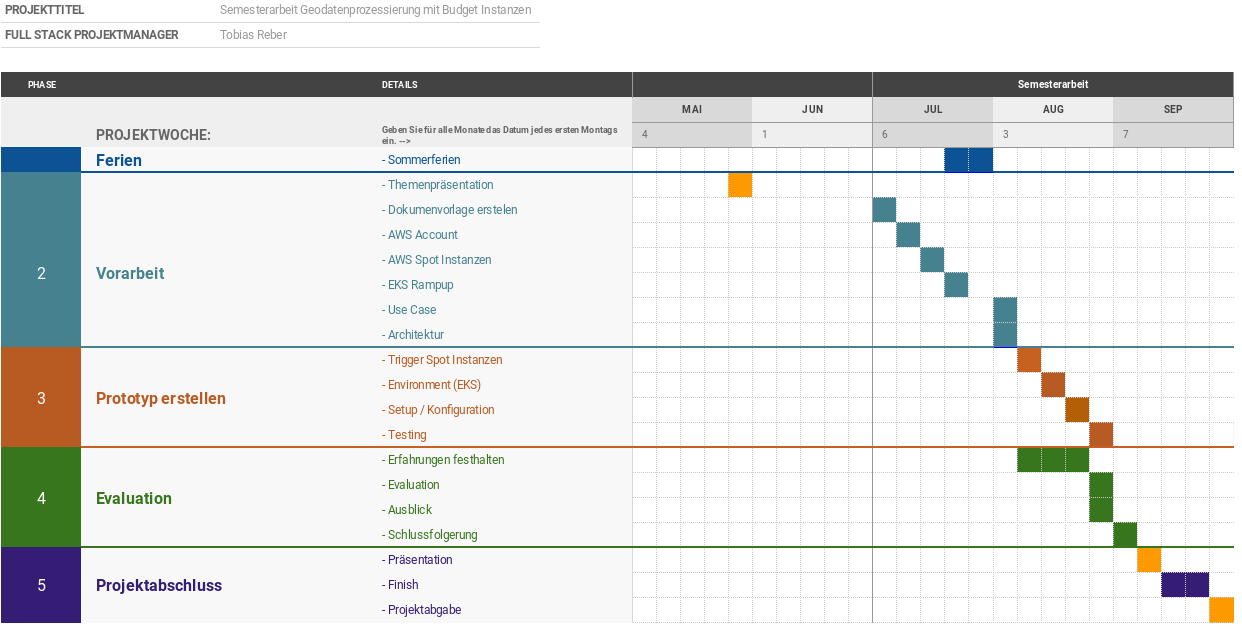
\includegraphics[width=.95\textwidth]{projektplanung}}
	\caption{\href{https://docs.google.com/spreadsheets/d/1zKTZgt4BW736G0xRfU9o3vWYwAJj-8nzFvGsPR7yJ_0/edit?usp=sharing}{Projektplan. Die orangen Meilensteine wurden von der BFH vorgegeben.}}
	\label{fig:Projektplan}
\end{figure}

\section{Konfigurationen und Kommandos}
\subsection{EFS auf EC2-Instanz mounten}
Anhand einer Anleitung, einem sogenannten Walktrough, wurde via AWS CLI\footnote{AWS Command Line Interface: Ein kommandozeilenorientiertes Werkzeug.} ein
EFS an eine EC2-Instanz gemountet und die Rohdaten wurden schon einmal dorthin kopiert. In der Verarbeitung bildet dieses EFS den Ausgang der Datenverarbeitung.
\appendCode{bash}{EFS auf EC2-Instanz mounten.}{src/walktrough_ec2_and_efs.sh}


\subsection{Von der SPOT Instanz aus abfragen, was ihr Status ist}\label{appendix:restful}
Von der Instanz aus können via RESTful API Metadaten der Instanz abgefragt werden. Bezüglich Interrupt einer Spot Instanz kann der Zustand \emph{none}, \emph{hibernate}, \emph{stop} oder \emph{terminate} sein. \emph{none}, wenn nichts ansteht. Von da an, wo klar ist, dass die Instanz abgestellt werden wird, kann der Zeitpunkt ausgelesen werden.
\appendCode{bash}{Status der Instanz abfragen}{src/rest_instance_metadata.sh}

\subsection{XML Testen}
Einfaches Skript, um zu testen, ob alle Dateien well-formed XML sind.
\appendCode{python}{XML testen}{src/up-and-running-dataprocessing/ansible/tests/test_xml_wellformed.py}

\subsection{Publikationsschritte in Ansible}
Der ganze Code zum hier aufgelisteten Ausschnitt kann auf \href{https://github.com/bfh-semesterarbeit/spot-geoprocessing}{github.com} eingesehen, resp. verwendet, werden:
\appendCode{make}{Nebst dem Setup werden die drei Publikationsschritte mit Ansible gesteuert.}{src/up-and-running-dataprocessing/ansible/playbooks/processing.yml}


%\section{Für die Semesterarbeit verwendete Software}
%\begin{itemize}
%\item JabRef: Verwaltung des Literaturverzeichnisses (BibTeX).
%\item Gummi: LaTeX Editor.
%\item AWS CLI: Für das Bereitstellen der AWS Infrastruktur.
%\item jq: Für das Filtern von JSON (vor allem von AWS CLI Antworten).
%\item git: Versionsmanagement der Textdateien.
%\item Google Spreadsheet: Für den \nameref{chap:projektplan}.
%\end{itemize}



%---------------------------------------------------------------------------
\end{document}
%---------------------------------------------------------------------------

